\documentclass{standalone}
\usepackage{graphicx}	
\usepackage{amssymb, amsmath}
\usepackage{color}

\usepackage{tikz}
\usetikzlibrary{intersections, backgrounds, math}
\usepackage{pgfmath}

\definecolor{light}{RGB}{220, 188, 188}
\definecolor{mid}{RGB}{185, 124, 124}
\definecolor{dark}{RGB}{143, 39, 39}
\definecolor{highlight}{RGB}{180, 31, 180}
\definecolor{light_teal}{RGB}{107, 142, 142}
\definecolor{mid_teal}{RGB}{72, 117, 117}
\definecolor{dark_teal}{RGB}{29, 79, 79}
\definecolor{gray10}{gray}{0.1}
\definecolor{gray20}{gray}{0.2}
\definecolor{gray30}{gray}{0.3}
\definecolor{gray40}{gray}{0.4}
\definecolor{gray60}{gray}{0.6}
\definecolor{gray70}{gray}{0.7}
\definecolor{gray80}{gray}{0.8}
\definecolor{gray90}{gray}{0.9}
\definecolor{gray95}{gray}{0.95}

\begin{document}

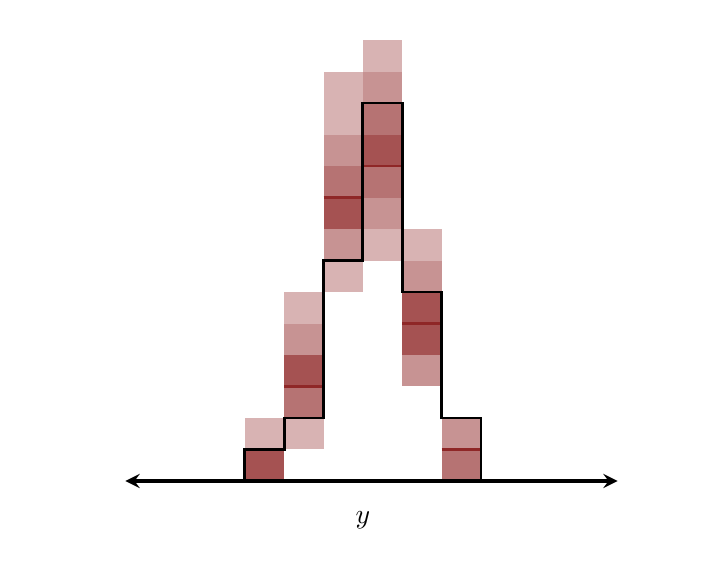
\begin{tikzpicture}[scale=1.0]

  \begin{scope}[shift={(0, 0)}]
    \draw[white] (-4.25, -3) rectangle (4.25, 3.75);

    \foreach \a/\b/\c/\d/\e/\f/\g/\h/\i/\j/\k [count=\n] in 
      {0.000/0.000/0.000/0.000/0.000/0.000/0.000/0.000/0.000/-3.000/-2.500, 
      0.000/0.000/0.000/0.000/0.000/0.000/0.000/0.000/0.000/-2.500/-2.000, 
      0.000/0.000/0.000/0.000/0.000/0.000/0.000/0.000/0.000/-2.000/-1.500, 
      0.000/0.000/0.000/0.000/0.000/1.000/1.000/1.000/2.000/-1.500/-1.000, 
      1.000/2.000/2.000/3.000/3.000/4.000/4.000/5.000/6.000/-1.000/-0.500, 
      6.000/7.000/8.000/8.000/9.000/9.000/10.000/11.000/13.000/-0.500/0.000, 
      7.000/8.000/9.000/10.000/10.000/11.000/12.000/13.000/14.000/0.000/0.500, 
      3.000/3.000/4.000/4.000/5.000/6.000/6.000/7.000/8.000/0.500/1.000, 
      0.000/0.000/0.000/1.000/1.000/1.000/1.000/2.000/2.000/1.000/1.500, 
      0.000/0.000/0.000/0.000/0.000/0.000/0.000/0.000/0.000/1.500/2.000, 
      0.000/0.000/0.000/0.000/0.000/0.000/0.000/0.000/0.000/2.000/2.500, 
      0.000/0.000/0.000/0.000/0.000/0.000/0.000/0.000/0.000/2.500/3.000} {
      \pgfmathsetmacro{\prop}{20 + 15 * 1};
      \colorlet{custom}{dark!\prop!white};
      \fill[custom] (\j, 0.4 * \a - 2) rectangle (\k, 0.4 * \i - 2);
      
      \pgfmathsetmacro{\prop}{20 + 15 * 2};
      \colorlet{custom}{dark!\prop!white};
      \fill[custom] (\j, 0.4 * \b - 2) rectangle (\k, 0.4 * \h - 2);
      
      \pgfmathsetmacro{\prop}{20 + 15 * 3};
      \colorlet{custom}{dark!\prop!white};
      \fill[custom] (\j, 0.4 * \c - 2) rectangle (\k, 0.4 * \g - 2);
      
      \pgfmathsetmacro{\prop}{20 + 15 * 4};
      \colorlet{custom}{dark!\prop!white};
      \fill[custom] (\j, 0.4 * \d - 2) rectangle (\k, 0.4 * \f - 2);
      
      \draw[dark, line width=1] (\j, 0.4 * \e - 2) -- (\k, 0.4 * \e - 2);
    };

    \draw[black, line width=1] (-3, -2)
    \foreach \x/\c in {-3.000/0.000, -2.500/0.000, -2.500/0.000, -2.000/0.000, 
                       -2.000/0.000, -1.500/0.000, -1.500/1.000, -1.000/1.000, 
                       -1.000/2.000, -0.500/2.000, -0.500/7.000, 0.000/7.000, 
                       0.000/12.000, 0.500/12.000, 0.500/6.000, 1.000/6.000, 
                       1.000/2.000, 1.500/2.000, 1.500/0.000, 2.000/0.000, 
                       2.000/0.000, 2.500/0.000, 2.500/0.000, 3.000/0.000} {
       -- (\x, 0.4 * \c - 2)
    };
     
    \draw [<->, >=stealth, line width=1.25] (-3.015, -2.00) -- +(6.25, 0);
    
    \node at (0, -2.5) { $y$ };
  \end{scope}
    
\end{tikzpicture}

\end{document}  